\documentclass[11pt,a4paper]{article}
\usepackage[top=3cm, bottom=2cm, left=2cm, right=2cm]{geometry}
\usepackage[utf8]{inputenc}
\usepackage{amsmath, amsfonts, amssymb}
\usepackage{siunitx}
\usepackage[brazil]{babel}
\usepackage{graphicx}
\usepackage[margin=10pt,font={small, it},labelfont=bf, textfont=it]{caption}
\usepackage[dvipsnames, svgnames]{xcolor}
\DeclareCaptionFont{MediumOrchid}{\color[svgnames]{MediumOrchid}}
\usepackage[pdftex]{hyperref}
\usepackage{natbib}
\bibliographystyle{plainnat}
\bibpunct{[}{]}{,}{s}{}{}
\usepackage{color}
\usepackage{footnote}
\usepackage{setspace}
\usepackage{booktabs}
\usepackage{multirow}
\usepackage{subfigure}
\usepackage{fancyhdr}
\usepackage{leading}
\usepackage{indentfirst}
\usepackage{wrapfig}
\usepackage{mdframed}
\usepackage{etoolbox}
\usepackage[version=4]{mhchem}
\usepackage{enumitem}
\usepackage{caption}
\usepackage{titlesec}
\usepackage{tcolorbox}
\usepackage{tikz}
\usepackage{LobsterTwo}
\usepackage[T1]{fontenc}
\usepackage{fontspec}
\usepackage{txfonts}
\AtBeginEnvironment{equation}{\fontsize{13}{16}\selectfont}


\titleformat{\section}{\LobsterTwo\LARGE\color{CarnationPink}}{\thesection.}{1em}{}
\titleformat{\subsection}{\LobsterTwo\LARGE\color{CarnationPink}}{\thesubsection}{1em}{}


\DeclareCaptionLabelFormat{figuras}{\textcolor{DarkTurquoise}{Figura \arabic{figure}}}
\captionsetup[figure]{labelformat=figuras}

\makeatletter
\renewcommand\tagform@[1]{\maketag@@@{\color{CarnationPink}(#1)}}
\makeatother

\renewcommand{\theequation}{Eq. \arabic{equation}}
\renewcommand{\thefigure}{Fig. \arabic{figure}}
\renewcommand{\thesection}{\textcolor{CarnationPink}{\arabic{section}}}

\setlist[itemize]{label=\textcolor{CarnationPink}{$\mathbf{\square}$}}

\setlist[enumerate]{label=\textcolor{CarnationPink}{\arabic*.}, align=left, leftmargin=1.5cm}


\newcounter{exemplo}

\NewDocumentEnvironment{exemplo}{ O{} }{%
\allowbreak
\setlength{\parindent}{0pt}
  \begin{mdframed}[
  leftline=true,
  topline=false,
  rightline=false,
  bottomline=false,
  linewidth=2pt,
  linecolor=CarnationPink,
  frametitlerule=false,
  frametitlefont=\LobsterTwo\large\color{CarnationPink},
  frametitle={\color{CarnationPink}\LobsterTwo\large #1},
  ]
}{%
  \end{mdframed}
}

\setlength{\fboxsep}{5pt}
\setlength{\fboxrule}{1.5pt}
\usepackage{float}
\renewcommand{\thefootnote}{\alph{footnote}}
\usepackage{url}
\hypersetup{
	colorlinks=true,
	linkcolor=DarkTurquoise,
	filecolor=DarkTurquoise,      
	urlcolor=DarkTurquoise,
	citecolor=DarkTurquoise,
	pdftitle={Especialista em Física da Radioterapia}
}
\pagestyle{fancy}
\fancyhf{}
\renewcommand{\headrulewidth}{0pt}
\rfoot{Página \thepage}

\title{\LobsterTwo\Huge{Radioterapia}}
\author{\LobsterTwo\Large{Teleterapia com Feixes de Elétrons}\nocite{*}}
\date{\LobsterTwo\textit{Dalila Mendonça}}
\begin{document}
	\maketitle

\section{Introdução}

	Feixes de elétrons têm sido usados em radioterapia desde a década de 1940, mas não ganharam uso generalizado até a década de 1970 com o desenvolvimento comercial dos aceleradores lineares (linacs). Os elétrons perdem energia à medida que atravessam um meio através de várias colisões elásticas e inelásticas com elétrons atômicos e o núcleo. Colisões inelásticas com o núcleo resultam na perda radiativa de um fóton, chamada produção de bremsstrahlung.
	
	A radiação bremsstrahlung criada pelas interações do feixe de elétrons com folhas de espalhamento de alto número atômico e outros materiais no caminho do feixe é chamada de contaminação de fótons. Os elétrons são uma partícula carregada com um alcance finito e, portanto, são adequados para o tratamento de alvos mais superficiais.

	Como se tratam de partículas carregadas, os elétrons de megavoltagem sofrem mais espalhamento do que os fótons de megavoltagem, particularmente no ar. É por isso que os feixes de elétrons usam cones com trimmers de feixe bem próximos à superfície do paciente para minimizar o espalhamento dos elétrons para fora do campo de tratamento. Para personalizar ainda mais a forma do feixe, os recortes cerrobend são colocados no topo dos trimmers (cutouts).

	O forma como ocorre o espalhamento dos elétrons muda com a energia inicial do elétron e com a profundidade no meio. Isso dificulta o matching de campos adjacentes de elétrons com outros campos de elétrons ou com campos de fótons. As muitas fontes de espalhamento no caminho do feixe de elétrons (folhas de espalhamento, câmaras monitoras, cone de elétrons) também afetam a dependência da distância da saída do feixe. O conceito de uma posição de fonte efetiva é usado para descrever isso.

	Três fatores que afetam grandemente a distribuição da dose dos feixes de elétrons são:
	
	\begin{enumerate}
		\item a obliquidade do feixe;
		\item a irregularidade da superfície; e
		\item a falta de homogeneidade do tecido.
	\end{enumerate}
	
	Os algoritmos pencil beam tradicionais não calculam com precisão a dose nessas condições. Os cálculos de Monte Carlo para elétrons estão se tornando cada vez mais comuns e funcionam muito melhor nessas condições.

	O AAPM TG-70, \textit{\textbf{``Recommendations for Clinical Electron Beam Dosimetry''}}, produziu um suplemento para o AAPM TG-25, \textit{\textbf{``Clinical Electron Beam Dosimetry''}}, que atualizou as seções de dosimetria absoluta para refletir a mudança na dose absorvida nos padrões de água. As discussões no AAPM TG-25 sobre obliquidade, dose de superfície, posição efetiva da fonte, correções de gap de ar e uso de diodos permanecem válidas. O relatório AAPM TG-70 apresenta uma discussão detalhada sobre o uso de elétrons em muitas situações clínicas.

\section{Características dos Feixes de Elétrons}

\subsection*{Porcentagem de Dose Na Profundidade}

	As curvas típicas de dose na profundidade para os feixe de elétrons são mostradas na \ref{fig:pdpeletrons}. Eles mostram uma dose de superfície relativamente alta em comparação com feixes de fótons com a mesma energia nominal, um acúmulo até a dose máxima, uma rápida queda na dose e, em seguida, um pequeno componente de baixa dose chamado cauda de bremsstrahlung ou contaminação de fótons. A contaminação de fótons aumenta com o aumento da energia, conforme mostrado na \ref{fig:pdpeletrons}.

	\begin{figure}[h]
		\centering
		\fcolorbox{DarkTurquoise}{white}{%
			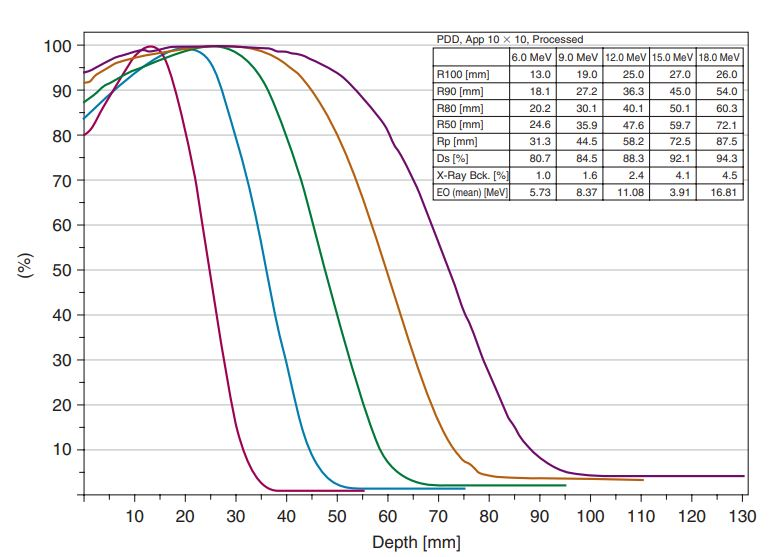
\includegraphics[width=0.6\textwidth]{Imagens/pdpeletrons.JPG}
		}%
		\caption{Exemplo de Curvas de PDP para feixes de Elétrons.}
		\label{fig:pdpeletrons}
	\end{figure}

	Existem vários parâmetros de dose na profundidade que são usados para descrever uma curva de dose de profundidade de elétrons: dose de superfície, profundidade de dose máxima (R100 ou $\mathrm{D_{max}}$), profundidade da isodose de 90\% (R90), profundidade da isodose de 80\% (R80), profundidade da isodose de 50\% (R50), alcance prático (Rp) e a contaminação por fótons.

	Os parâmetros de alcance das isodoses na profundidade mudam com o tamanho do campo, mas a mudança é pequena para tamanhos de campo maiores do que o alcance prático. De fato, os dados na literatura demonstram que para energias menores ou iguais a 16 MeV, as mudanças em qualquer um dos parâmetros de alcance são menores que 1 mm para os cones de 10 cm x 10 cm até os cones de 25 cm x 25 cm. Para energias menores ou iguais a 12 MeV, isso se estende até o cone de 6 cm x 6 cm. Um exemplo da alteração do R90 em função do tamanho de campo é apresentado na \ref{fig:r90}.
	
	\begin{figure}[h]
		\centering
		\fcolorbox{DarkTurquoise}{white}{%
			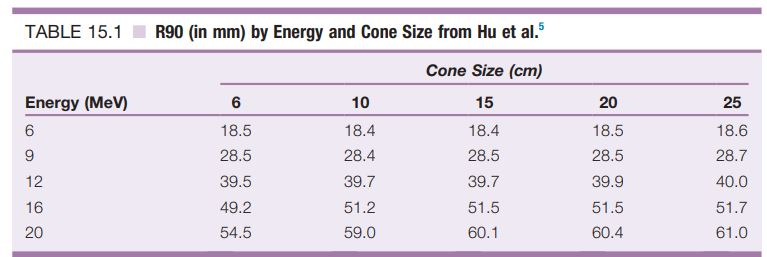
\includegraphics[width=0.6\textwidth]{Imagens/r90.JPG}
		}%
		\caption{R90 (em mm) em função da energia e do tamanho do cone.}
		\label{fig:r90}
	\end{figure}
	
	Para energias mais altas pode haver diferenças significativas, como mostra a \ref{fig:pdpeletronsECampo}. Para elétrons, a dose de superfície aumenta com a energia, o que é o oposto de fótons, e também pode ser observado na \ref{fig:pdpeletrons}.

	\begin{figure}[h]
		\centering
		\fcolorbox{DarkTurquoise}{white}{%
			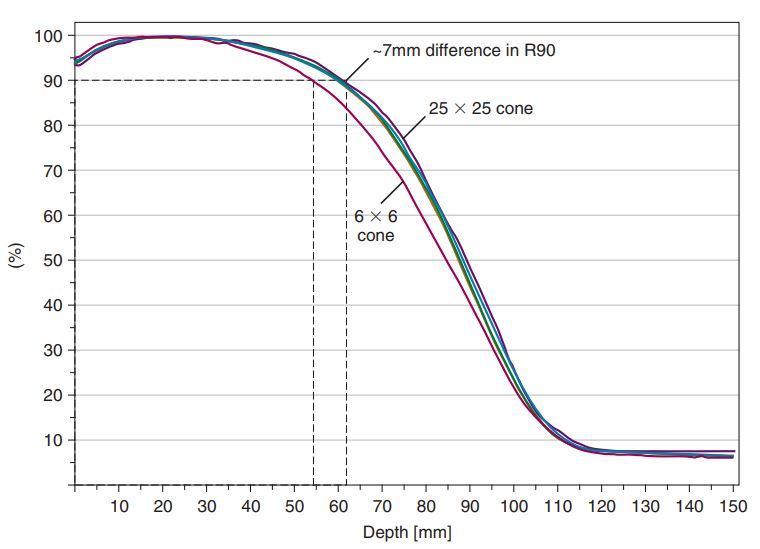
\includegraphics[width=0.5\textwidth]{Imagens/pdpeletronsECampo.JPG}
		}%
		\caption{Exemplo de mudança da PDP com diminuição do tamanho do cone para um elétron de maior energia (22 MeV).}
		\label{fig:pdpeletronsECampo}
	\end{figure}

	A \ref{fig:estimarOsRs} apresenta regras gerais que podem ser usadas para estimar os parâmetros de alcance. Estas regras destinam-se a ser estimativas rápidas e não podem substituir os dados medidos. Os valores podem diferir ligeiramente entre os linacs de diferentes modelos. Na prática clínica, esses valores devem ser tabelados em um formato conveniente semelhante à tabela da \ref{fig:pdpeletrons} e disponibilizados prontamente aos médicos como um auxílio na escolha da energia do feixe. Na prática clínica, a energia é frequentemente selecionada de modo que a profundidade R90 seja no mínimo tão profunda quanto o a região mais distal do volume alvo (PTV). A energia também deve ser limitada para reduzir a dose em quaisquer tecidos ou órgãos de risco (OARs) distais ao alvo.

	\begin{figure}[h]
		\centering
		\fcolorbox{DarkTurquoise}{white}{%
			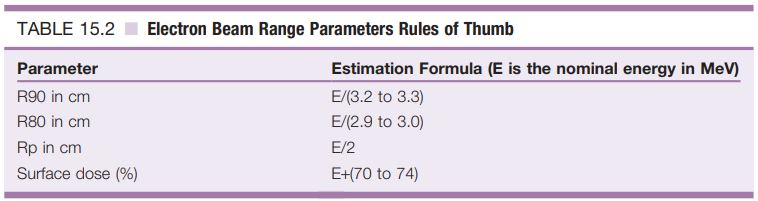
\includegraphics[width=0.8\textwidth]{Imagens/estimarOsRs.JPG}
		}%
		\caption{Regras práticas para estimar os parâmetros de alcance do feixe de elétrons.}
		\label{fig:estimarOsRs}
	\end{figure}

\subsection*{Output e Cutouts}

	A tendência de output dos cones de elétrons varia de acordo com a energia. O Centro de Física Radiológica (RPC), agora IROC Houston, publicou dados de referência para muitos modelos de linacs. Um exemplo do conjunto de dados é mostrado na \ref{fig:fatorcone}. Como pode-se observar, a PDP permanece inalterada para tamanhos de campo maiores do que o alcance prático. Da mesma forma, há pouca mudança no output de um feixe de elétrons para tamanhos de cutout iguais ao alcance prático. Dado que Rp pode ser estimado como E/2, isso implica que apenas campos menores que 3 cm em um feixe de 6 MeV terão mudanças significativas. Este valor é apenas uma estimativa, e sua validade para um determinado acelerador deve ser estabelecida no momento do comissionamento.

	O AAPM TG-70 descreve um método para estimar a dose na profundidade e o output para cutouts retangulares de dimensão $X \times Y$ por meio da média geométrica, dada por:

	\begin{equation}
		OF_{X,Y} = \left(OF_X \times OF_Y\right)^{\frac{1}{2}}
	\end{equation}

	\begin{equation}
		PDP_{X,Y} = \left(PDP_X \times PDP_Y\right)^{\frac{1}{2}}
	\end{equation}

	\begin{wrapfigure}{r}{0.5\textwidth}
		\centering
		\fcolorbox{DarkTurquoise}{white}{%
			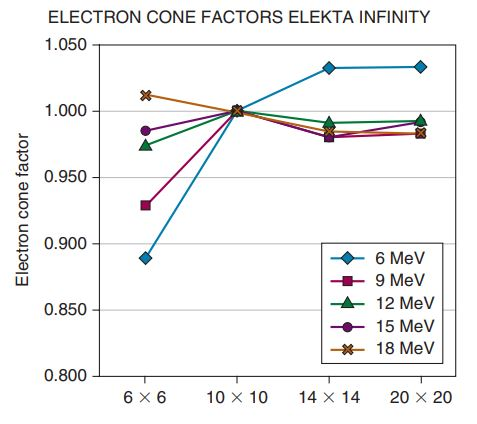
\includegraphics[width=0.4\textwidth]{Imagens/fatorcone.JPG}
		}%
		\caption{Exemplo de fatores de output do cone de elétrons em função do tamanho do cone e da energia do feixe.}
		\label{fig:fatorcone}
	\end{wrapfigure}

	Estas equações requerem que sejam realizadas medidas de uma série de cutouts no momento do comissionamento. Embora funcione para cutouts retangulares, estas equações não são particularmente precisas para cutouts pequenos ou com formatos irregulares. Khan descreveu um método baseado no conceito de proporção de buildup lateral (LBR) que descreve com mais precisão as alterações no output e na dose na profundidade. O LBR é derivado da razão entre a PDP para um cutout de 2 cm de diâmetro e a PDP para o cone aberto. Para cutouts irregulares, um método de integração setorial é usado para calcular a PDP e o output. Estes cálculos são facilmente implementados em códigos de programação, mas é difícil de serem utilizados em um cálculo manual. Kehwar e Huq propuseram uma melhoria neste método. Na prática, cutouts pequenos ou irregulares devem ser medidos para confirmar o output e a PDP.

	Para cutouts pequenos, a curva de dose na profundidade se deslocará em direção à superfície, conforme mostrado na Figura 15.4. Portanto, tanto o output de dose quanto a PDP devem ser verificadas, pois isso pode alterar a escolha da energia. A Figura 15.4 também mostra que o efeito é mais enunciado em energias mais altas, como esperado.

	\begin{figure}[h]
		\centering
		\subfigure{
			\fcolorbox{DarkTurquoise}{white}{%
				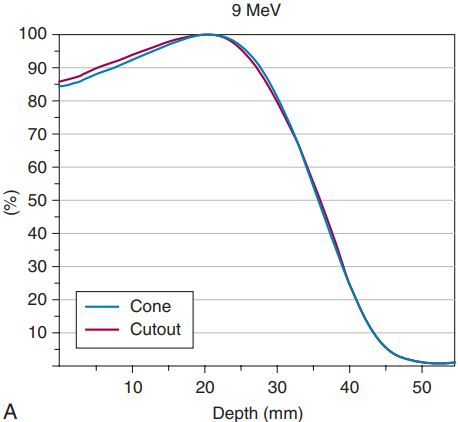
\includegraphics[width=0.4\textwidth]{Imagens/cutoutA.JPG}
			}
			\fcolorbox{DarkTurquoise}{white}{%
				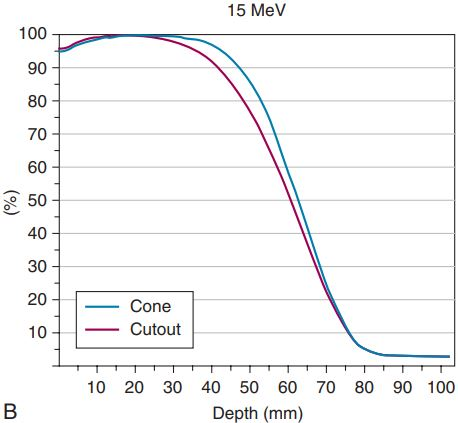
\includegraphics[width=0.4\textwidth]{Imagens/cutoutB.JPG}
			}} \\ %structures.
		\caption{A mudança na PDP para um cutout menor que o a abertura do conveniente(4 cm).}
		\label{fig:cutout}
	\end{figure}

	A forma das curvas de isodose para feixes de elétrons também depende da energia e da profundidade. A \ref{fig:cobertura90cutouts} mostra, para várias energias, a largura da curva de 90\%, a profundidade proximal e a profundidade distal para os cutouts de tamanhos 2 cm x 9 cm, 4 cm x 9 cm e 9 cm x 9 cm colocados em um cone cone de 10 cm x 10 cm .
	
	\begin{figure}[h]
		\centering
		\fcolorbox{DarkTurquoise}{white}{%
			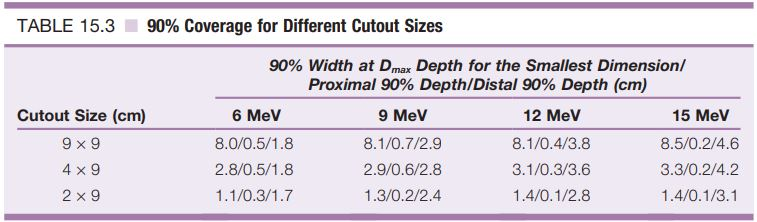
\includegraphics[width=0.8\textwidth]{Imagens/cobertura90cutouts.JPG}
		}%
		\caption{Cobertura de 90\% para diferentes tamanhos de cutouts.}
		\label{fig:cobertura90cutouts}
	\end{figure}
	
	
	A largura da curva de 90\% é medida na profundidade da dose máxima. Os dados mostram que a margem necessária para o cutout é de cerca de 1 cm. Deve-se observar que a largura da curva de 90\% diminui significativamente com a profundidade e a profundidade distal da curva de 90\% torna-se muito mais rasa para energias mais altas à medida que o tamanho do cutout diminui. Portanto, o planejamento computadorizado do tratamento é recomendado para garantir a cobertura ideal no alvo, como mostra a \ref{fig:isodoseCutout}. 
	
	\begin{figure}[h]
		\centering
		\fcolorbox{DarkTurquoise}{white}{%
			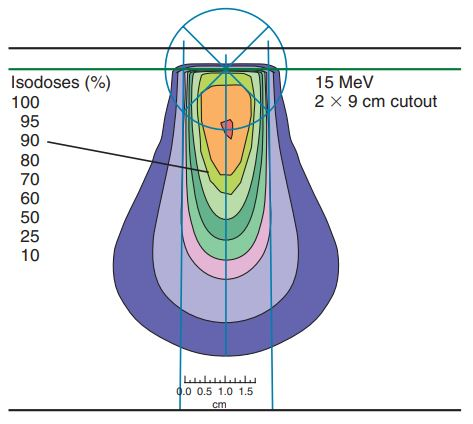
\includegraphics[width=0.5\textwidth]{Imagens/isodoseCutout.JPG}
		}%
		\caption{Linhas de isodose para um cutout estreito para um feixe de elétrons de alta energia.}
		\label{fig:isodoseCutout}
	\end{figure}
	
	A colimação de chumbo sobre a pele às vezes é usada para campos pequenos, uma vez que a penumbra é relativamente larga em comparação com o tumor. A colimação da pele também pode fornecer uma melhor proteção das estruturas superficiais próximas. A espessura dos cutouts e colimações devem ser suficientes para reduzir a transmissão para menos de 5\%. Caso for usado chumbo, uma boa regra para definir a espessura necessária em mm é E/2; caso for usado cerrobend, o valor obtido para o chumbo deve ser multiplicado por um fator de 1.2 (TG-25).

\subsection*{Penumbra}

	A penumbra de um feixe de elétrons é uma função da energia feixe e da profundidade. A Comissão Internacional de Unidades e Medidas de Radiação (ICRU) recomenda que a penumbra seja definida como a distância do ponto de 80\% ao ponto de 20\% em um perfil de feixe. o ICRU também recomenda que a penumbra seja determinada na profundidade de R85/2. A penumbra aumenta com a profundidade para todas as energias, com energias mais altas mostrando os aumentos mais acentuados. A \ref{fig:penumbraEletrons} mostra um exemplo de medidas da penumbra. As mudanças drásticas da penumbra com a profundidade dificultam o matching de campos adjacentes.

	\begin{figure}[h]
		\centering
		\fcolorbox{DarkTurquoise}{white}{%
			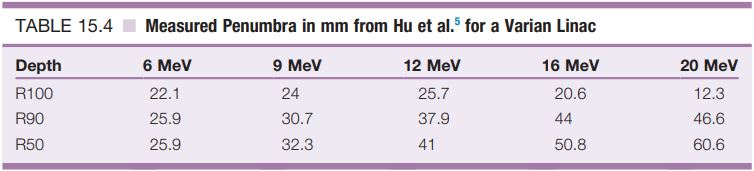
\includegraphics[width=0.8\textwidth]{Imagens/penumbraEletrons.JPG}
		}%
		\caption{Penumbra medida em mm para um Acelerador da Varian.}
		\label{fig:penumbraEletrons}
	\end{figure}

\subsection*{SSD Extendida}

	Como o espalhamento aumenta com a distância entre o cone e a superfície do paciente, o output e a penumbra também irão mudar para uma distância extendida da fonte até a superfície (SSDs). Um estudo mostrou um aumento de 8 mm a 10 mm na penumbra para um feixe de 6 MeV para uma SSD de 110 cm. As múltiplas fontes de espalhamento no caminho do feixe de elétrons causam uma dependência entre o  cone/cutout e a energia com o output e a SSD. Ao plotar a mudança no output em função à SSD, pode-se obter a SSD efetiva ($SSD_{eff}$), que pode então ser usado para calcular o output do feixe de elétrons para uma SSD arbitrária. As medidas podem ser feitas para a SSD de 100 cm, 110 cm e 120 cm, por exemplo. 


	\begin{tcolorbox}[width=\textwidth, colback={white}, colbacktitle={DarkTurquoise!50!white}, title={$\bigstar$ \LobsterTwo{Determinação da $\mathbf{SSD_{eff}}$} $\bigstar $}, coltitle={CarnationPink}, colframe={DarkTurquoise}, fonttitle=\rmfamily\bfseries\Large]

		Se \textcolor{DarkTurquoise}{$\mathbf{I_0}$} é a leitura em \textcolor{DarkTurquoise}{$\mathbf{d_{max}}$} para um gap de ar \textcolor{DarkTurquoise}{$\mathbf{gap = 0}$}, ou seja, para SSD nominal do feixe (padronizada em $SSD_0 = 100$ cm); e \textcolor{DarkTurquoise}{$\mathbf{I_g}$} é a leitura em \textcolor{DarkTurquoise}{$\mathbf{d_{max}}$} para um gap de ar \textcolor{DarkTurquoise}{$\mathbf{g}$}, de modo que \textcolor{DarkTurquoise}{$\mathbf{SSD = SSD_0 + g}$}; Plotando um gráfico de \textcolor{DarkTurquoise}{$\mathbf{\left(I_0 / I_g\right)^{1/2}}$} em função de \textcolor{DarkTurquoise}{$\mathbf{g}$} será criada uma linha reta com inclinação igual a \textcolor{DarkTurquoise}{$\mathbf{b = 1 / (SSD_{eff} + d_{max})}$} e portanto a SSD efetiva será dada por \textcolor{DarkTurquoise}{$\mathbf{SSD_{eff} = (1/b) - d_{max}}$}.

	\end{tcolorbox}

	Para tratamentos com a SSD extendida, aplica-se a lei do inverso quadrado utilizando a $\mathbf{SSD_{eff}}$ ao invés da SSD nominal de calibração fornecida pelo telêmero, de modo que o fator do inverso quadrado $ISF$ é dado por:

	\begin{equation}
		ISF = \left(\frac{SSD_{eff}}{SSD_{eff} + \Delta SSD}\right)^2
	\end{equation}

	\begin{exemplo}[onde,]
		\begin{itemize}
			\item \textcolor{DarkTurquoise}{\textbf{\Delta SSD}} é a variação entre a $SSD_0$ e a SSD estendida para o qual deseja-se obter o fator ISF.
		\end{itemize}
	\end{exemplo}

	A dose $D_g$ com gap de ar $g = \Delta SSD$ pode então ser determinada a partir da dose $D_0$ fornecida com um gap de ar $g = 0$, na profundidade de dose máxima através da seguinte equação:

	\begin{equation}
		D_g = D_0 \left(\frac{SSD_{eff} + d_{max}}{SSD_{eff} + \Delta SSD + d_{max} }\right)^2
	\end{equation}
	
	O gráfico de $(I_0/I_g)^{1/2}$ versus $g$ será linear apenas até uma SSD extendida de aproximadamente 115 cm. Em maiores SSDs, a mudança no output deve ser determinada através de medições. Como alternativa, uma série de medições podem ser feitas durante o comissionamento para utilizar como referência futura. O AAPM TG-25 afirma que a correção utilizando a SSD efetiva não varia com a profundidade e toda as curvas de dose na profundidade podem ser corrigidas utilizando o mesmo fator de correção, o que significa que a PDP não muda significativamente com a SSD, pelo menos até a SSD de 115 cm.

\section{Superfícies Irregulares e Obliquidade}

	A obliquidade do feixe e a irregularidade da superfície estão intimamente relacionadas, pois ambas envolvem a incidência do feixe em ângulos não normais (plano da superfície não é paralelo ao plano ortogonal à direção de incidência do feixe). Como por padrão, os dados da dosimetria são medidos para uma incidência normal, devem ser feitas correções caso utilize feixes oblíquos. Para ângulos de incidência inferiores a \ang{30}, as correções devido a obliquidade são pequenas, onde as curvas de isodose são meramente deslocadas paralelamente à superfície. Para ângulos iguais ou superiores a \ang{30}, três mudanças são observadas, como mostra a \ref{fig:obliquidade}:

	\begin{enumerate}
		\item Um aumento na dose perto de $d_{max}$;
		\item Deslocamento da profundidade terapêutica ($\approx$ 90\%) em direção à superfície; e
		\item Aumento da dose nas profundidades oblíquas próximas ao alcance prático.
	\end{enumerate}


	\begin{figure}[h]
		\centering
		\subfigure{
			\fcolorbox{DarkTurquoise}{white}{%
				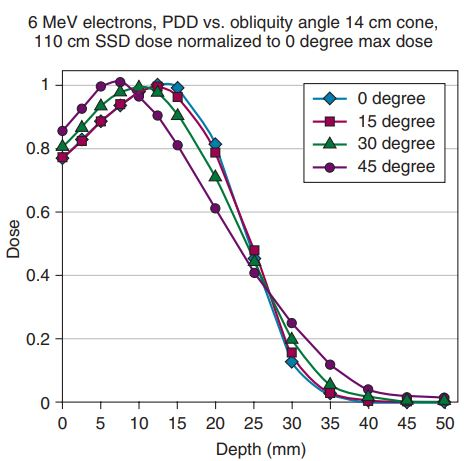
\includegraphics[width=0.4\textwidth]{Imagens/obliquidadeA.JPG}
			}}
		\subfigure{
			\fcolorbox{DarkTurquoise}{white}{%
				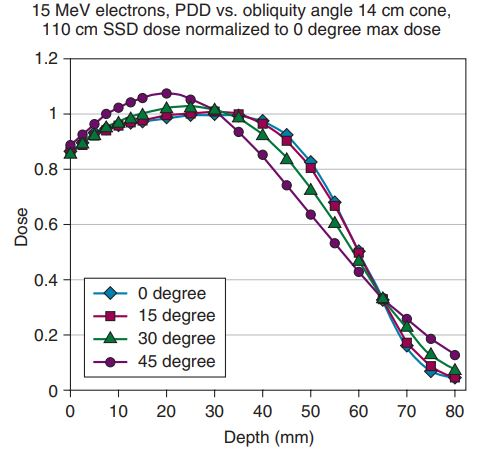
\includegraphics[width=0.4\textwidth]{Imagens/obliquidadeB.JPG}
			}} \\ %
		\caption{Efeito da obliquidade em feixes de elétrons.}
		\label{fig:obliquidade}
	\end{figure}

	As superfícies arredondadas (irregulares/ não planas) afetam a dose na profundidade de modo que as isodoses são deslocadas para mais perto da superfície à medida que a obliquidade ao longo feixe muda gradualmente, como mostra a \ref{fig:efeitoSuperficieirregular}.

	\begin{figure}[h]
		\centering
		\fcolorbox{DarkTurquoise}{white}{%
			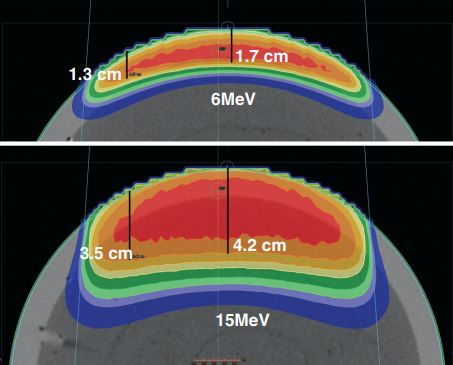
\includegraphics[width=0.5\textwidth]{Imagens/efeitoSuperficieirregular.JPG}
		}%
		\caption{Efeito de superfícies arredondadas em feixes de elétrons.}
		\label{fig:efeitoSuperficieirregular}
	\end{figure}

	Já os casos de protuberâncias teciduais (como, o nariz) ou déficits teciduais (como, déficits cirúrgicos) são uma forma de irregularidades na superfície que possuem um efeito semelhante ao causado devido a heterogeneidades no meio. Nestes casos, dado a interface entre dois tecidos com diferentes densidades, os pontos quentes serão formados no lado da interface que possui menor densidade, como mostra a \ref{fig:hotspots}.
	
	\begin{figure}[h]
		\centering
		\subfigure{
			\fcolorbox{DarkTurquoise}{white}{%
				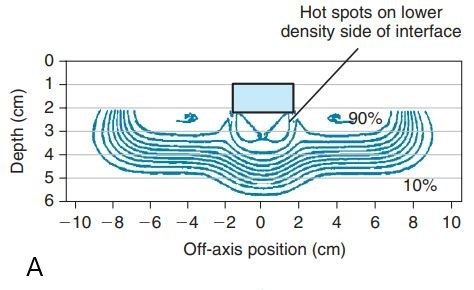
\includegraphics[width=0.4\textwidth]{Imagens/hotspots1.jpg}
			}}
		\subfigure{
			\fcolorbox{DarkTurquoise}{white}{%
				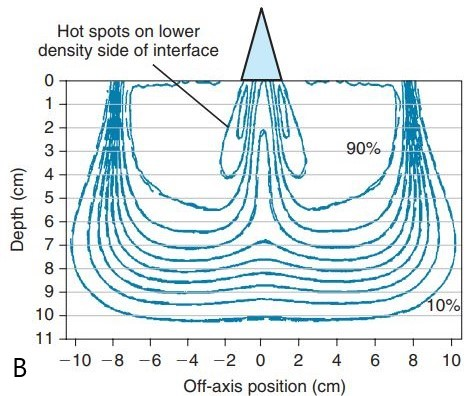
\includegraphics[width=0.4\textwidth]{Imagens/hotspots2.JPG}
			}} \\ %
		\caption{Demonstração de pontos quentes no lado de baixa densidade das interfaces teciduais. A figura \textbf{A} mostra uma cavidade de baixa densidade dentro de um phantom de água. A figura \textbf{B} mostra uma protuberância com densidade de água criando uma região de menor densidade adjacente a ela.}
		\label{fig:hotspots}
	\end{figure}


\section{Heterogeneidades}

	Existem duas preocupações com a falta de homogeneidade do tecido: a atenuação e o espalhamento. A atenuação causada por uma região heterogênea pode ser estimada calculando-se o coeficiente de espessura equivalente (CET - \textit{ coefficient of equivalent thickness} ). O CET é aproximadamente igual à razão entre o poder de freamento da região heterogênea e o poder de freamento da água e pode ser estimado pela razão das densidades eletrônicas de cada meio. A dose em uma profundidade $d$ localizado além de uma heterogeneidade é determinada calculando a profundidade efetiva na água $d_{eff}$, de modo que para estimar a dose na profundidade $d$ é utilizada a PDP para $d_{eff}$. Deve-se enfatizar que esta é apenas uma estimativa e um TPS devidamente comissionado é altamente recomendado para calcular com precisão as doses para regiões heterogêneas. A ($d_{eff}$) é obtida através da equação:

	\begin{equation}
		d_{eff} = d - t(1 - CET)
	\end{equation}

	\begin{exemplo}
		\begin{itemize}
			\item \textcolor{DarkTurquoise}{$\mathbf{d}$} é a profundidade nominal (espessura) do ponto onde deseja-se determinar a dose;
			\item \textcolor{DarkTurquoise}{$\mathbf{t}$} é a espessura da profundidade heterogênea;
			\item \textcolor{DarkTurquoise}{$\mathbf{CET}$} é o coeficiente de espessura equivalente, cujos valores típicos são:
				\begin{itemize}[label=\textcolor{CarnationPink}{$\star$}]
					\item \textcolor{MediumOrchid}{\textbf{Osso:}} $CET \approx 1.65$
					\item \textcolor{MediumOrchid}{\textbf{Pulmão:}} $CET \approx 0.33$
				\end{itemize}
		\end{itemize}
	\end{exemplo}

	Como ja citado anteriormente, pode-se observar na \ref{fig:heterogeneidade}  que os pontos quentes se formam lateralmente à interface heterogênea no lado do tecido de menor densidade. Isso se deve ao aumento do espalhamento no material de maior densidade no sentido do material de menor densidade que não é compensado pelo espalhamento no material de baixa densidade.

	\begin{figure}[h]
		\centering
		\subfigure{
			\fcolorbox{DarkTurquoise}{white}{%
				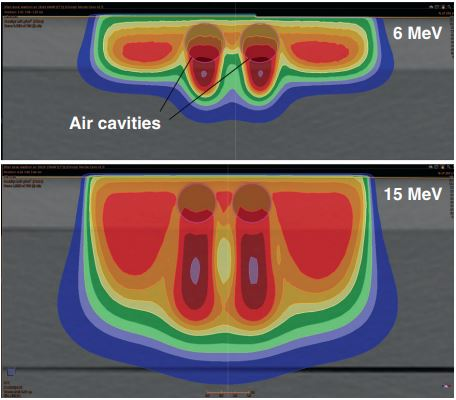
\includegraphics[width=0.4\textwidth]{Imagens/heterogeneidadenoArEletrons.JPG}
			}}
		\subfigure{
			\fcolorbox{DarkTurquoise}{white}{%
				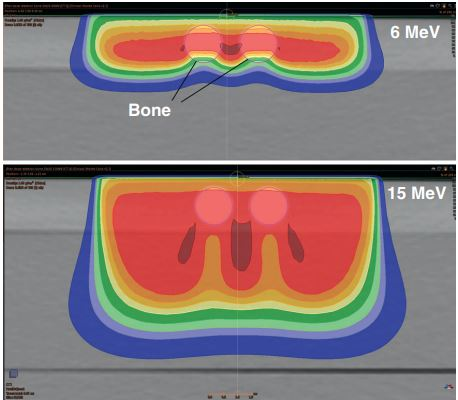
\includegraphics[width=0.4\textwidth]{Imagens/heterogeneidadeOssoEletrons.JPG}
			}} \\ %
		\caption{Efeitos da heterogeneidade devido a um meio de ar e a um meio de osso.}
		\label{fig:heterogeneidade}
	\end{figure}

\section{Bolus e Compensadores}

	Os Bolus podem ser usados com feixes de elétrons por três razões:

	\begin{enumerate}
		\item Para aumentar a dose na superfície;
		\item Para compensar as irregularidades na superfície;
		\item Para moldar a isodose (distal) para se conformar/adequar ao PTV;
	\end{enumerate}
	
	As doses na superfície variam de 70\% a 90\% da dose de prescrição, dependendo do modelo do acelerador e da energia do feixe. Para atingir a dose recomendada para cobertura do PTV de 90\%, a maior parte das energias exigirá algum bolus caso o PTV tenha uma parte superficial. 
	
	Muitos materiais estão disponíveis para serem utilizados como bolus, como a cera de parafina, poliestireno, acrílico, Super-Stuff, Superflab, Superflex e folhas termoplásticas (ambos descritos no Tg-70). A cera de parafina (cera odontológica), o poliestireno e acrílico são trabalhosos para serem  e moldados. Os produtos ``Super'' são flexíveis e podem se moldar à superfície da pele, mas podem ser difíceis de usar para cobrir grandes áreas curvas sem formar  abaulamentos. Se cobertos com filme plástico diariamente, podem ser reutilizados. As folhas termoplásticas têm a vantagem de poder cobrir grandes áreas sem formar abaulamentos. Porém, a menos que o paciente seja posicionado exatamente da mesma forma todos os dias, pode ser difícil obter a mesma conformidade com a pele. É improvável que gaps de ar de até 10 mm afetem significativamente a dose na superfície, mas caso houver suspeita de que haja gaps de ar consideráveis, o paciente deve ser ``escaneado'' com o bolus na sua posição correta para confirmar a extensão do gap de ar ou então um novo bolus deve ser ser construído. Uma revisão mais recente de materiais de bolus discutem materiais adicionais, como Play-Doh, gaze úmida com água ou vaselina, entre outros.

	O bolus também pode ser usado para preencher espaços vazios, afim de se eliminar possíveis pontos quentes e frios causados pela presença da cavidades de ar, como o canal auditivo externo ou as vias nasais. A cera odontológica é normalmente utilizada nesses casos. A água foi proposta para o canal auditivo, mas pode ser desconfortável para o paciente. 

	Os compensadores podem ser usados para preencher déficits teciduais, construir uma superfície para torná-la mais uniforme ou moldar a região distal da curva de isodose para cobrir o PTV. Os déficits teciduais podem ser preenchidos com moldes de cera, vaselina ou faixas de folhas de óleo gel. Por exemplo, para um tratamento de nariz, um molde de cera pode ser criado para nivelar a superfície e eliminar os pontos quentes que irão se formar semelhantes aqueles demonstrados na \ref{fig:hotspots}.

	Se o PTV não estiver em uma profundidade uniforme, uma determinada energia de elétron comprometerá a cobertura ou tratará um excesso de tecido normal. Um  bolus compensador personalizado pode ser criado adicionando o material sobre as áreas de menor profundidade do PTV para deslocar a isodose em direção à superfície, conforme mostrado na Figura 15.11. Isso pode ser feito manualmente por meio de um processo de tentativa e erro. Neste caso, o paciente deverá ser tomografado com o bolus final posicionado em seu devido lugar e o planejamento computadorizado deve ser realizado para confirmar a cobertura do PTV. Devem ser evitados regiões acentuadas na superfície do compensador (protuberâncias) para não produzir pontos quentes. Uma empresa (.decimal) desenvolveu um processo para usinar o compensador de forma personalizada com base na superfície do paciente, no formato do PTV e na energia do feixe de elétrons, de modo que seja um processo muito menos demorado e mais preciso.

\section{Blindagem de Estruturas Adjacentes}

	Se um OAR estiver adjacente ao campo de tratamento, pode ser necessário colocar uma blindagem diretamente no paciente para ``afiar'' a borda do campo e proteger a estrutura. Esta blindagem é particularmente importante em SSDs estendidas, onde o espalhamento para fora do campo aumenta. Exemplos de regiões que utilizam as blindagens são o cristalino, as glândulas lacrimais e o interior da boca.
	
	Embora 3 mm a 5 mm de chumbo possam ser suficientes para proteger os tecidos subjacentes (abaixo da blindagem), uma blindagem interna pode causar um aumento significativo na dose nos tecidos sobrejacentes (acima da blindagem) devido ao retroespalhamento. O retroespalhamento aumenta com o aumento do número atômico da blindagem e diminui com o aumento da energia do elétron. De acordo com a equação fornecida no AAPM TG-25, é estimado que o retroespalhamento pode ser de até 60\%. Um cálculo mais moderno mostrou que o retoespalhamento está na faixa de 20\% a 50\%, dependendo da energia do elétron. Para minimizar os efeitos do retroespalhamento, deve ser usado uma blindagem laminada posicionando os materiais em ordem crescente com respeito ao número atômico. Por exemplo, a camada proximal pode ser de cera, seguida por uma camada de alumínio e, em seguida, pode ser usada uma camada de chumbo. O projeto de qualquer blindagem deve ser validado com medidas para certificar sua eficácia.

\section{Considerações Clínicas Gerais}

	O AAPM TG-70 tem uma série de seções sobre situações clínicas que vão desde mama intacta, parede torácica, nariz, olho, couro cabeludo e parótidas. Algumas semelhanças gerais percorrem essas seções, sendo as principais:

	\begin{enumerate}[label=\textcolor{CarnationPink}{(\roman*)}]
		\item O planejamento de tratamento computadorizado é altamente recomendado, particularmente para campos adjacentes, campos oblíquas, superfícies irregulares e meios heterogêneos. Um algoritmo pencil beam pode ter limitações significativas nessas situações e, portanto, um algoritmo mais moderno como Monte Carlo é preferível.
		\item As margens dos cutouts devem levar em consideração a penumbra e o movimento respiratório. Para pequenos cutouts, pode ser necessário aumentar as margens, principalmente para energias mais altas.
		\item Se os campos forem adjacentes, recomenda-se que a junção seja movida pelo menos uma vez durante o tratamento para minimizar os pontos quentes e frios.
		\item A dosimetria in vivo e no phantom deve ser realizada para validar setups complicados.
		\item É necessário uma boa imobilização para os casos de setup complicados.
		\item O bolus personalizado é recomendado para superfícies irregulares, para déficits de tecido e para moldar as linhas de isodose distais de acordo com o PTV. Como as doses de superfície do feixe de elétrons variam de 70\% a 90\%, o bolus quase sempre será necessário se houver uma componente superficial do PTV. O bolus deve ter pelo menos 2 cm de largura para evitar um ponto frio sob o bolus.
		\item As blindagens oculares projetadas para tratamentos de fótons não devem ser usadas para elétrons.
	\end{enumerate}

\section{Novas Tendências}

	Embora os fundamentos dos tratamentos com feixes de elétrons tenham permanecido inalterados desde a década de 1970, existem várias técnicas emergentes, incluindo arcos, colimadores de múltiplas folhas de elétrons (eMLC), modulação de energia e terapia de radiação modulada por intensidade de elétrons/fótons (IMRT).

	Os arcos de elétrons são usados por alguns centros há muito tempo, mas não foram amplamente implementados devido à sua complexidade. Como os cones padrão, com uma distância típica de 95 cm até os trimmers, causariam uma colisão durante um arco, é necessário um cone personalizado ou a utilização dos jaws colimadores, onde a largura deve ser de 4 cm a 8 cm. Se a curvatura da superfície mudar na direção superior-inferior, uma largura cônica (afunilada) pode ser usada. A blindagem na superfície é necessária por dois motivos: para ``afiar'' a borda do feixe, pois os trimmers padrão do cone não são usados, e para permitir a uniformidade no início e no final do arco. A dose na superfície é menor para os tratamentos de arco porque as áreas mais próximas ao isocentro são expostas a maiores segmentos de arco. A componente de contaminação com fótons também aumentará na profundidade, pois o feixe está focado no isocentro.  

	Vários estudos examinaram o desenvolvimento de MLCs de elétrons. Eles propõem que isso eliminará o tempo de fabricação dos recortes, eliminará a exposição da equipe a um material perigoso (cerrobend) e permitirá o IMRT para elétrons. Resta saber se o custo e a complexidade do comissionamento de tais sistemas os tornarão amplamente aceitos na prática clínica.

	O IMRT de elétrons através do uso da modulação de energia também foi investigado. Existe um produto comercial disponível (Trumpet eIMRT, Standard Imaging) que determinará uma combinação de energias de feixe com base na homogeneidade de dose desejada sobre o PTV e o bolus a ser usado. 
	
	Um report descreveu o uso de campos IMRT de feixe de fótons em combinação com feixes de elétrons para reduzir a penumbra, melhorar a uniformidade da dose no PTV e reduzir as doses nos OARs.

\bibliography{ref.bib}
\end{document}